% LTeX: language=de-DE
\section{Virtuelle Maschine}

\begin{frame}{Virtuelle Maschine}
	\begin{itemize}
		\item Meistens: Eine \emph{Virtuelle Maschine} (VM) simuliert echte Computer
		      \begin{itemize}
			      \item Display
			      \item Lautsprecher
			      \item Festplatte
			      \item \dots
		      \end{itemize}
		\item Hier: Software, die wie die CPU eines Rechners funktioniert
	\end{itemize}
\end{frame}

\begin{frame}{Wie eine CPU Programme ausführt \TODO{DELETE}}
	\begin{itemize}
		\item Die meisten Prozessoren basieren auf der \emph{von Neumann Architektur}~\scite[p.~172]{Ledin2020-yp}
		\item Eine CPU enthält nach von Neumann ein \emph{Rechenwerk}\footnote{Engl: \enquote{arithmetic logic unit} (ALU).}, \emph{Steuerwerk}\footnote{Engl: \enquote{control unit}.}, \emph{Speicherwerk}, \emph{Ein- / Ausgabewerk} und ein Bussystem~\scite[p.~172]{Ledin2020-yp}
		\item Die Programmausführung wird durch den sog. \emph{Befehlszyklus}\footnote{Engl: \enquote{fetch-decode-execute cycle}.} modelliert~\scite[pp.~208-209]{Ledin2020-yp}:
		\item[] \begin{enumerate}
				\item \textbf{Fetch} (Befehl laden): Das Steuerwerk lädt die nächste Anweisung aus dem Speicher
				\item \textbf{Decode} (Befehl dekodieren): Der Befehlscode und die Operanden werden ermittelt
				\item \textbf{Execute} (Befehl ausführen): Die zuständige Einheit im Prozessor wird verwendet, um den Befehl zu verarbeiten.
				      Beispielsweis wird das Rechenwerk für logische und mathemtische Befehle aufgerufen.
			\end{enumerate}
	\end{itemize}
\end{frame}

\begin{frame}{Übertragung der Konzepte auf die rush VM \TODO{DELETE}}
	\Lirsting[ranges={16-26}, caption={Struct Definition der VM.}, label={lst:vm_struct}, fancyvrb={fontsize=\footnotesize}, float=H]{deps/rush/crates/rush-interpreter-vm/src/vm.rs}
	\begin{itemize}
		\item \TODO{fix broken caption}
		\item \qVerb{stack}: Speicher für temporäre Werte bei komplexeren Operationen
		\item \qVerb{mem}: Anhaltender Speicher mit einer festen Größe für Variablen
		\item \qVerb{mem_ptr}: Hält den Index der letzten freien Speicherzelle in \qVerb{mem}
		\item \qVerb{call_stack}: Aufrufstapel, welcher den \emph{Befehlsähler} und den \emph{Funktionszähler} für jeden Aufruf speichert
	\end{itemize}
\end{frame}

\begin{frame}{Speicherstruktur der rush VM. \TODO{DELETE}}
	\begin{itemize}
		\item Unterscheidung zwischen zwei Arten der Adressierung
		\item \emph{relative Adressierung}: \qVerb{svari *rel[0]}
		\item \emph{absolute Adressierung}: \qVerb{svari *abs[0]}
	\end{itemize}

	\begin{figure}
		\centering
		\begin{NiceTabular}{>{\scriptsize}c}[name=Left]
			\\
			\\
			\\
			num              \\
			\Block[draw]{} 9 \\
		\end{NiceTabular}\hspace{1cm}
		\begin{NiceTabular}
			[
				first-col,
				%code-for-first-col=\ValueMinusOne{iRow},
				first-row,
				hvlines,
				colortbl-like,
				name = Right
			]
			{cc>{\scriptsize}c}
			 & cell                  & rel    & {\normalsize abs} \\
			 & a                     & $-3$   & $mp + rel = 0$    \\
			 & b                     & $-2$   & $mp + (-2) = 1$   \\
			 & c                     & $-1$   & $mp - 1 = 2$      \\
			 & d                     & $0$    & $3$               \\
			 & \cellcolor{gray!30} e & $1$    & $mp + 1 = 4$      \\
			 & \ldots                & \ldots & \ldots            \\
		\end{NiceTabular}

		\begin{tikzpicture}[overlay,remember picture]
			\draw [->] (Left-5.5-|Left-last) to [bend left] (Right-5.5-|Right-1);
			\draw [thick, dashed] (Right-4.5-|Right-5) --  node[anchor=west, xshift=-1cm, align=center] {\scriptsize memory\\ \scriptsize pointer $= 3$} ([xshift=2.5cm]Right-4.5-|Right-4);
		\end{tikzpicture}
		\caption{Speicherstruktur der rush VM.}\label{fig:rush_vm_linmem}
	\end{figure}
\end{frame}

\begin{frame}{Ein Beispielprogramm der rush VM \TODO{Delete}}
	\hspace{0pt} % This is somehow required
	\vfill
	\Lirsting[caption={Beispielprogramm der rush VM.}, fancyvrb={fontsize=\footnotesize}, float=H]{deps/paper/listings/vm_faster_instructions.s}
	\vfill
\end{frame}

\begin{frame}{Struktur der Programme der rush VM}
	\begin{itemize}
		\item Stack für temporäre Operationen
		\item Weiterer Stack für Funktionsaufrufe
		\item Unterteilung in Funktionen
		      \begin{itemize}
			      \item Ohne Namen
			      \item numerische Identifizierung
			      \item Enthält mehrere Anweisungen
		      \end{itemize}
		\item Git Commit \enquote{\rushCommit{}}: ca.\ 30 verschiedene Befehlscodes
		\item Struktur der Anweisungen: \enquote{\LirstInline{asm}{call 2}}
		      \begin{itemize}
			      \item Befehlscode (\texttt{call})
			      \item Optionaler Operand (\texttt{2})
		      \end{itemize}
	\end{itemize}
\end{frame}

\begin{frame}{VM: Fazit}
	\begin{itemize}
		\item Ca. 2.7 mal schneller als der Tree-walking Interpreter
		\item Einfache Implementierung des Compilers
		      \begin{itemize}
			      \item  Stack-basierte Architektur
			      \item Gleichzeitige Entwicklung von VM und Compiler
			      \item Hoher Abstraktionsgrad
		      \end{itemize}
	\end{itemize}
\end{frame}

\begin{frame}{Demonstration: Eingabe}
	\Lirsting[float=H, fancyvrb={frame=none, fontsize=\footnotesize}]{listings/pow.rush}
\end{frame}

\begin{frame}{Demonstration: Ausgabe}
    \Lirsting[float=H, fancyvrb={frame=none, fontsize=\footnotesize}, ranges={1-16,+8 60-71}]{listings/vm_pow_rush.s}
\end{frame}

\begin{frame}{Demonstration: Laufzeitverhalten}
	\begin{center}
		\href{run:assets/01_rush_presentation_vm.mp4}{
			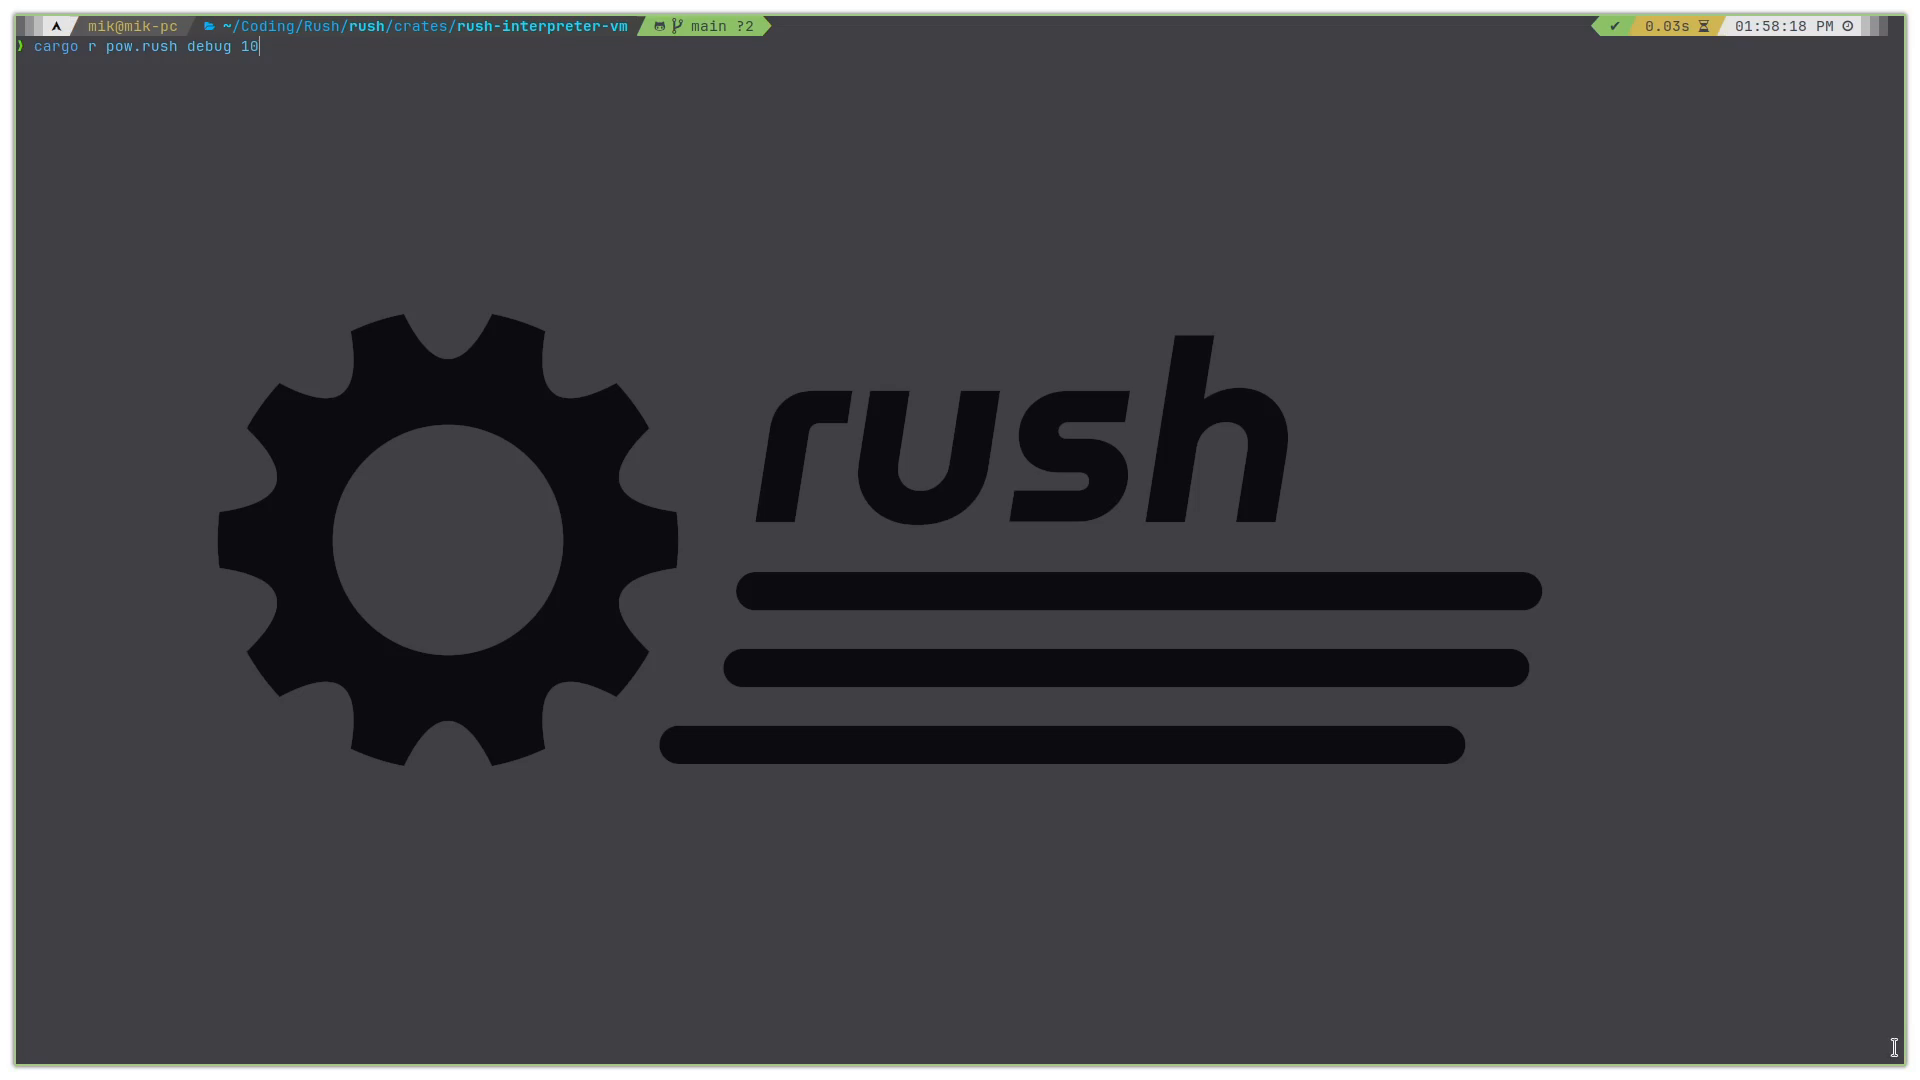
\includegraphics[width=\textwidth]{assets/01_rush_presentation_vm.png}
		}
	\end{center}
\end{frame}
